\section{Các Bài toán Khác: Ước tính Tư thế và Theo dõi Đối tượng}
\label{sec:other_core_tasks}

\subsection{Tổng quan}
\label{subsec:pose_tracking_overview}
Vượt ra ngoài việc nhận dạng và khoanh vùng các đối tượng tĩnh, thị giác máy tính hiện đại còn đi sâu vào việc phân tích cấu trúc và hành vi động. Hai trong số những bài toán cốt lõi và có tác động lớn nhất trong lĩnh vực này là \textbf{Ước tính Tư thế (Pose Estimation)} và \textbf{Theo dõi Đối tượng (Object Tracking)}. Chúng không chỉ trả lời câu hỏi "Cái gì ở đâu?", mà còn mở rộng ra "Nó có cấu trúc như thế nào?" và "Nó đang di chuyển ra sao?".

Việc giải quyết các bài toán này cho phép các hệ thống AI không chỉ "nhìn thấy" thế giới một cách thụ động, mà còn có khả năng \textbf{hiểu được cấu trúc, chuyển động, và hành vi} của con người cũng như vật thể trong không gian và thời gian. Điều này là nền tảng cho vô số các ứng dụng tương tác và tự hành, từ robot cộng tác, thực tế tăng cường, đến phân tích thể thao và giám sát an ninh thông minh.

\subsection{Ước tính Tư thế (Pose Estimation)}
\label{subsec:pose_estimation}
\textbf{Định nghĩa:} Ước tính tư thế là bài toán dự đoán vị trí (tọa độ 2D hoặc 3D) của một tập hợp các \textbf{điểm khớp (keypoints)} hoặc "khớp" (joints) trên một đối tượng, phổ biến nhất là cơ thể người. Các keypoints này tạo thành một "bộ xương" (skeleton) biểu diễn cấu trúc và tư thế của đối tượng.

\begin{center}
	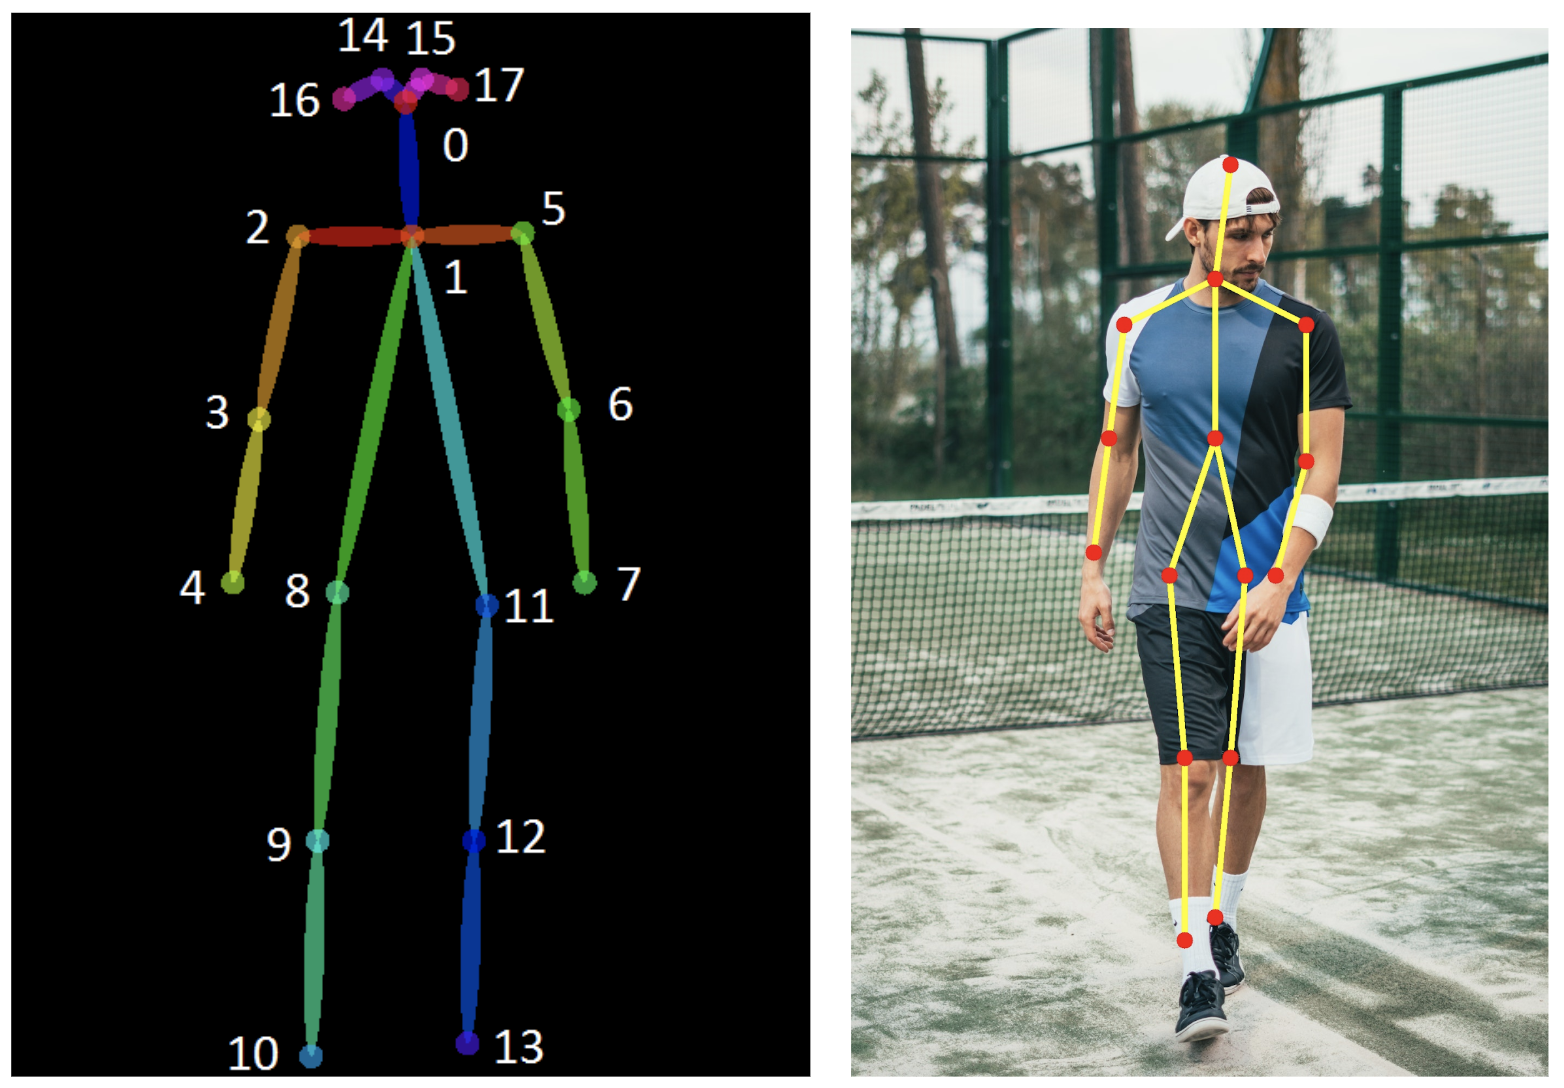
\includegraphics[width=0.8\textwidth]{images/human_pose_estimation_keypoints.png}
	\captionof{figure}{Ví dụ về Ước tính Tư thế Người. Mô hình dự đoán tọa độ của các điểm khớp chính (mắt, vai, khuỷu tay, cổ tay, hông, đầu gối, mắt cá chân) và kết nối chúng để tạo thành một bộ xương ảo.}
	\label{fig:pose_estimation_keypoints}
\end{center}
% Keyword gợi ý: human pose estimation keypoints, skeleton estimation

\subsubsection{Các Phương pháp Tiếp cận Chính}
\label{subsubsec:pose_estimation_approaches}
Có hai hướng tiếp cận chính cho bài toán ước tính tư thế:
\begin{enumerate}
	\item \textbf{Top-down (Từ trên xuống):} Đầu tiên, sử dụng một bộ phát hiện vật thể (object detector) để khoanh vùng từng người trong ảnh. Sau đó, một mô hình ước tính tư thế cho một người duy nhất (single-person pose estimator) được áp dụng trên từng vùng đã khoanh để tìm các keypoints. Cách tiếp cận này thường cho độ chính xác cao nhưng tốc độ phụ thuộc vào bộ phát hiện và có thể thất bại nếu không phát hiện được người ban đầu.
	\item \textbf{Bottom-up (Từ dưới lên):} Đầu tiên, mô hình phát hiện tất cả các keypoints có thể có trong toàn bộ ảnh (ví dụ, tất cả các "khuỷu tay", tất cả các "đầu gối"). Sau đó, một thuật toán gom nhóm (grouping/parsing) được sử dụng để kết nối các keypoints này lại thành các bộ xương của từng người. Cách tiếp cận này thường nhanh hơn và bền bỉ hơn trong các cảnh đông người.
\end{enumerate}

\subsubsection{Các Mô hình Tiêu biểu}
\label{subsubsec:pose_estimation_models}

\paragraph{OpenPose (2017): Bottom-up với PAFs} 
\textbf{OpenPose} \cite{Cao2017} là mô hình bottom-up tiên phong, cho phép ước tính tư thế nhiều người trong thời gian thực. Điểm đột phá cốt lõi là \textbf{Part Affinity Fields (PAFs)}.

\textbf{Toán học cốt lõi:}  
Giả sử có $K$ loại keypoints (ví dụ: vai, khuỷu tay, đầu gối,...) và $C$ loại limbs (chi nối các keypoints). Mạng dự đoán:
\begin{align}
	H_k(x,y) &= \text{heatmap}(x,y) \quad \forall k \in \{1,\dots,K\} \\
	L_c(x,y) &= \text{PAF}(x,y) \in \mathbb{R}^2 \quad \forall c \in \{1,\dots,C\}
\end{align}
Trong đó $H_k$ cho biết xác suất keypoint $k$ tại vị trí $(x,y)$, và $L_c$ là vector chỉ hướng của limb $c$.  

\textbf{Loss function:} Mạng được huấn luyện bằng:
\begin{equation}
	\mathcal{L} = \sum_{k} \| H_k - \hat{H}_k \|_2^2 + \sum_{c} \| L_c - \hat{L}_c \|_2^2,
\end{equation}
trong đó $\hat{H}_k, \hat{L}_c$ là ground-truth heatmaps và PAFs.  

\textbf{Trực giác:} PAFs giúp mạng học \textit{liên kết không gian} giữa các keypoints. Khi ghép các điểm keypoints đã phát hiện, ta tích hợp thông tin vector PAF dọc theo limb để chọn cặp keypoints phù hợp, tức là mô hình học \textbf{hướng và cấu trúc cơ thể con người}.

---

\paragraph{HRNet (2019): Giữ Độ phân giải Cao}
\textbf{HRNet} \cite{Sun2019} giải quyết hạn chế của CNN truyền thống là giảm độ phân giải làm mất chi tiết. 

\textbf{Kiến trúc và toán học:}  
HRNet duy trì $M$ luồng song song với các độ phân giải khác nhau $\{R_1, \dots, R_M\}$, với $R_1$ cao nhất. Tại mỗi tầng $t$, feature maps được cập nhật bằng:
\begin{equation}
	F_i^{(t+1)} = f_i(F_i^{(t)}) + \sum_{j \neq i} \text{Resize}_{R_i \leftarrow R_j}(g_j(F_j^{(t)})),
\end{equation}
trong đó $f_i$ là conv block nội tại, $g_j$ là mapping giữa các luồng, và $\text{Resize}_{R_i \leftarrow R_j}$ là phép up/down-sampling.  

\textbf{Trực giác:} Luồng độ phân giải cao giữ thông tin vị trí chi tiết (precise spatial cues), luồng thấp cung cấp ngữ cảnh rộng. Fusion liên tục giúp mô hình dự đoán keypoints chính xác hơn, đặc biệt khi keypoints gần nhau hoặc bị che khuất.

---

\paragraph{ViTPose (2022): Transformer cho Pose Estimation}
\textbf{ViTPose} \cite{Xu2022} áp dụng Vision Transformer trực tiếp vào bài toán pose estimation.

\textbf{Cách huấn luyện:}  
1. Ảnh được chia thành các patch $\{x_1, \dots, x_N\}$ và ánh xạ thành embedding $\{z_1, \dots, z_N\}$ bằng patch embedding.
2. Transformer xử lý embedding với self-attention:
\begin{equation}
	Z' = \text{Transformer}(Z) \in \mathbb{R}^{N \times D},
\end{equation}
giúp mỗi token "nhìn" được toàn bộ ảnh và nắm quan hệ giữa các keypoints.
3. Token đầu ra được biến đổi thành heatmaps $H_k$ cho từng keypoint thông qua head tuyến tính:
\begin{equation}
	H_k = \text{Linear}_k(Z').
\end{equation}

\textbf{Loss function:} Thường dùng MSE giữa heatmap dự đoán và ground-truth, tương tự HRNet.

\textbf{Trực giác:} Self-attention cho phép mô hình học \textbf{quan hệ toàn cục} giữa các khớp, xử lý tốt trường hợp che khuất hoặc tư thế khó. Khác với CNN truyền thống, ViTPose không giới hạn receptive field, do đó dễ học các cấu trúc cơ thể phức tạp.

\textbf{Tóm tắt tư duy chung:}
\begin{itemize}
	\item OpenPose: Học các trường vector để nối keypoints → tập trung vào cấu trúc địa phương (local connectivity).
	\item HRNet: Giữ và trao đổi đa độ phân giải → cân bằng chi tiết không gian và ngữ cảnh.
	\item ViTPose: Transformer học quan hệ toàn cục → nắm cấu trúc phức tạp và che khuất.
\end{itemize}

\subsection{Theo dõi Đối tượng (Object Tracking)}
\label{subsec:object_tracking}

\textbf{Định nghĩa:} Theo dõi đối tượng (Object Tracking) là bài toán xác định vị trí và duy trì danh tính (ID) của một hoặc nhiều đối tượng trong chuỗi video, tức là một bài toán 4D: không gian 2D + thời gian + ID.  

\textbf{Bản chất toán học:}  
Tại khung hình $t$, giả sử tập các detection là $\mathcal{D}_t = \{d_1^t, \dots, d_{N_t}^t\}$, và tập các track hiện tại là $\mathcal{T}_{t-1} = \{T_1^{t-1}, \dots, T_M^{t-1}\}$. Nhiệm vụ là tìm ánh xạ:
\[
\phi: \mathcal{D}_t \rightarrow \mathcal{T}_{t-1} \cup \{\text{new ID}\},
\]
sao cho tổng chi phí liên kết được tối ưu, ví dụ:
\[
\phi^* = \arg \min_\phi \sum_{i} \text{cost}(T_{\phi(d_i)}, d_i),
\]
trong đó cost có thể dựa trên khoảng cách không gian, đặc trưng ngoại hình, hoặc dự đoán chuyển động.

---

\subsubsection{Tracking-by-Detection: Mô thức thống trị}
\label{subsubsec:tracking_by_detection}

Hầu hết MOT hiện đại tuân theo pipeline:
\begin{enumerate}
	\item \textbf{Detection:} Tại mỗi frame $t$, sử dụng bộ phát hiện vật thể (YOLO, Faster R-CNN, v.v.) để thu thập $\mathcal{D}_t$.
	\item \textbf{Data Association:} Liên kết các detection với các track hiện có $\mathcal{T}_{t-1}$ bằng một hàm chi phí (cost function) đa chiều:
	\[
	\text{cost}(T_i, d_j) = \lambda_1 \text{IoU}(T_i, d_j) + \lambda_2 \text{cosine}(f(T_i), f(d_j)) + \lambda_3 \text{motion}(T_i, d_j)
	\]
	với $f(\cdot)$ là feature ngoại hình và motion là dự đoán vị trí từ bộ lọc Kalman.
\end{enumerate}

---

\subsubsection{Các Mô hình Hiện đại}
\label{subsubsec:tracking_models}

\paragraph{DeepSORT (2018):} \cite{Wojke2017}  
Mở rộng SORT bằng cách bổ sung đặc trưng ngoại hình (appearance feature).  

\textbf{Cấu trúc:}
\begin{itemize}
	\item \textbf{Motion Model:} Bộ lọc Kalman dự đoán vị trí $(x,y,w,h)$:
	\[
	\hat{x}_t = A x_{t-1} + \epsilon, \quad \epsilon \sim \mathcal{N}(0, Q)
	\]
	Chi phí liên kết giữa detection $d_j$ và track $T_i$ dựa trên khoảng cách Mahalanobis:
	\[
	d_{\text{motion}}^2 = (d_j - \hat{x}_t)^T S^{-1} (d_j - \hat{x}_t)
	\]
	\item \textbf{Appearance Model:} Mạng CNN trích xuất feature $f(d_j) \in \mathbb{R}^D$. Chi phí liên kết:
	\[
	d_{\text{appearance}} = 1 - \frac{f(d_j) \cdot f(T_i)}{\|f(d_j)\|\|f(T_i)\|}
	\]
	\item \textbf{Matching Cascade:} Giải bài toán gán ghép bằng thuật toán Hungarian tối ưu tổng chi phí:
	\[
	\min \sum_{i,j} \mathbf{1}_{\text{match}}(i,j) \big(d_{\text{motion}} + d_{\text{appearance}}\big)
	\]
\end{itemize}

---

\paragraph{ByteTrack (2021):} \cite{Zhang2022}  
Giải quyết vấn đề false negatives từ detection có độ tin cậy thấp bằng cơ chế \textbf{two-stage association}.

\textbf{Cơ chế:}
\begin{enumerate}
	\item Chia detections thành \textit{high-confidence} $\mathcal{D}^H$ và \textit{low-confidence} $\mathcal{D}^L$.
	\item Bước 1: Liên kết các track hiện có với $\mathcal{D}^H$.
	\item Bước 2: Liên kết các track còn lại với $\mathcal{D}^L$ để phục hồi các đối tượng bị che khuất.
\end{enumerate}

\textbf{Chi phí liên kết:} Thường dựa trên IoU hoặc Kalman prediction:
\[
\text{cost}(T_i, d_j) = 1 - \text{IoU}(\hat{b}_i, b_j)
\]

\textbf{Trực giác:}  
Giữ lại các detection có độ tin cậy thấp giúp giảm false negatives và ID switches, đặc biệt trong môi trường đông người hoặc khi có che khuất.

\begin{center}
	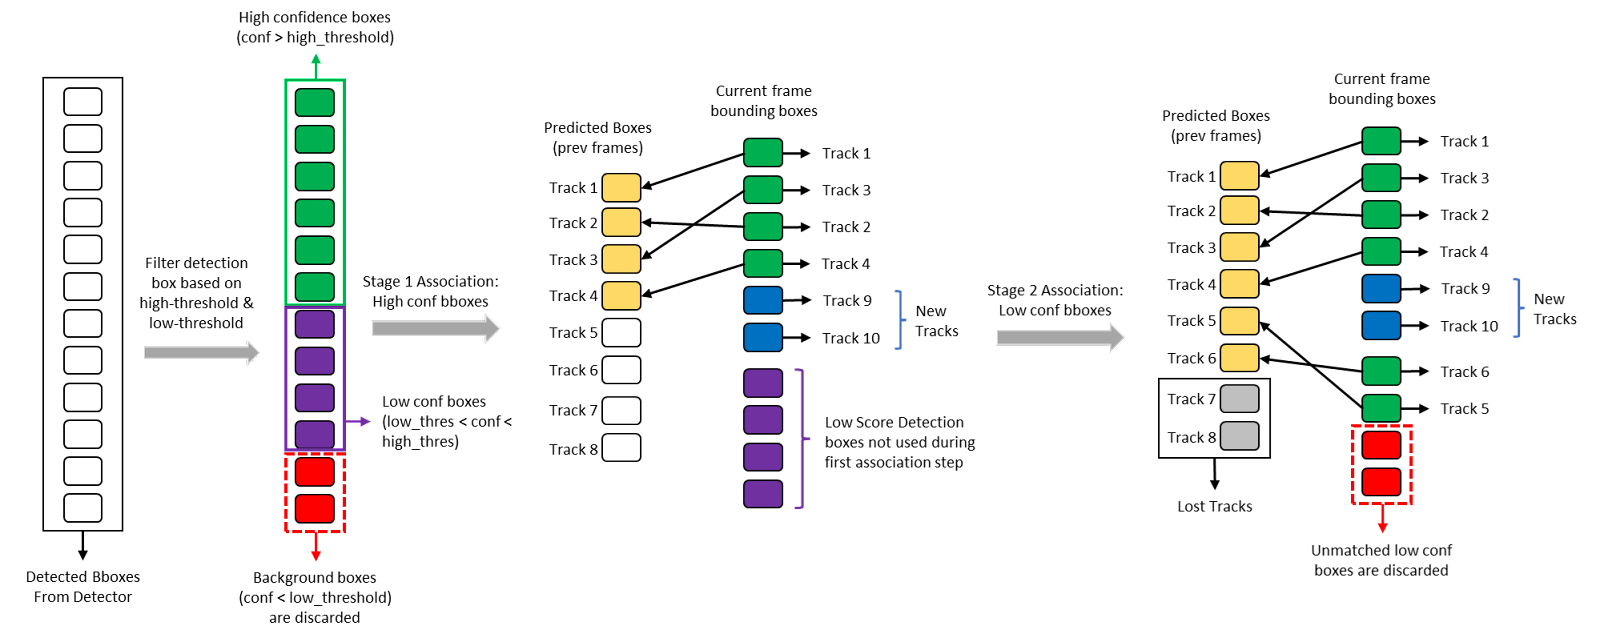
\includegraphics[width=0.8\textwidth]{images/bytetrack_matching_principle.png}
	\captionof{figure}{Nguyên lý ByteTrack: hai bước liên kết với detections high-confidence và low-confidence, giúp duy trì track ngay cả khi đối tượng bị che khuất.}
	\label{fig:bytetrack_principle}
\end{center}

---

\paragraph{Xu hướng mới (2023-2025):}  
\begin{itemize}
	\item \textbf{Transformer-based MOT:} Mô hình như \textbf{MOTR} dùng attention để học trực tiếp các tương quan giữa object queries qua thời gian.
	\item \textbf{OC-SORT:} Sử dụng motion model phức tạp hơn, kết hợp \textit{orientation-aware} và Kalman mở rộng.
	\item \textbf{BoT-SORT:} Tích hợp feature ngoại hình mạnh mẽ hơn (có thể từ CLIP), kết hợp motion model tinh vi.
	\item \textbf{Unified tracking:} Xu hướng tích hợp phân đoạn, nhận dạng hành vi, và theo dõi trong một pipeline duy nhất, hướng tới các hệ thống "Tracking Anything" tương tự SAM/DINO cho video.
\end{itemize}

\textbf{Trực giác tổng thể:}  
Object Tracking là sự cân bằng giữa:
\begin{itemize}
	\item Dự đoán động học (motion) → giữ track khi đối tượng tạm thời che khuất.
	\item Đặc trưng ngoại hình (appearance) → phân biệt các đối tượng giống nhau.
	\item Detections đa mức tin cậy → giảm false negatives và ID switches.
\end{itemize}

\subsection{Kết luận: Hướng tới Nhận thức Động học và Hành vi}
\label{subsec:pose_tracking_conclusion}
Cả Ước tính Tư thế và Theo dõi Đối tượng đều là những bước tiến quan trọng, đưa thị giác máy tính từ việc nhận thức các khung cảnh tĩnh sang việc hiểu được một thế giới động. Chúng cung cấp cho máy móc khả năng diễn giải không chỉ "ai" và "cái gì" đang ở đâu, mà còn "họ đang làm gì" và "sẽ di chuyển như thế nào tiếp theo".

Sự phát triển từ các phương pháp kinh điển như OpenPose và DeepSORT đến các kiến trúc hiện đại dựa trên Transformer như ViTPose và các thuật toán liên kết thông minh như ByteTrack cho thấy một xu hướng rõ ràng: hướng tới các hệ thống AI có khả năng \textbf{nhận thức động học và hành vi} một cách toàn diện. Đây chính là nền tảng cho thế hệ tiếp theo của các ứng dụng thông minh, từ robot tương tác, xe tự hành, đến các hệ thống phân tích thể thao và y tế phục hồi chức năng.

\section*{Tài liệu tham khảo}
\begin{itemize}
	\item[1] Cao, Z., Simon, T., Wei, S. E., \& Sheikh, Y. (2017). Realtime multi-person 2d pose estimation using part affinity fields. In \textit{Proceedings of the IEEE conference on computer vision and pattern recognition (CVPR)}. (Paper gốc giới thiệu OpenPose).
	\item[2] Sun, K., Xiao, B., Liu, D., \& Wang, J. (2019). Deep high-resolution representation learning for human pose estimation. In \textit{Proceedings of the IEEE/CVF conference on computer vision and pattern recognition (CVPR)}. (Paper gốc giới thiệu HRNet).
	\item[3] Xu, Y., Zhang, Q., Zhang, J., \& Tao, D. (2022). Vitpose: Simple vision transformer baselines for human pose estimation. In \textit{Advances in Neural Information Processing Systems (NeurIPS)}. (Paper gốc giới thiệu ViTPose).
	\item[4] Wojke, N., Bewley, A., \& Paulus, D. (2017). Simple online and realtime tracking with a deep association metric. In \textit{2017 IEEE international conference on image processing (ICIP)}. (Paper gốc giới thiệu DeepSORT).
	\item[5] Zhang, Y., Sun, P., Jiang, Y., Yu, D., Weng, F., Yuan, Z., ... \& Wang, X. (2022). Bytetrack: Multi-object tracking by associating every detection box. In \textit{European conference on computer vision (ECCV)}. (Paper gốc giới thiệu ByteTrack).
	\item[6] Cao, J., Weng, L., Jiang, X., Yang, Y., \& Yuan, Y. (2023). Observation-centric sort: Rethinking sort for robust multi-object tracking. \textit{arXiv preprint arXiv:2203.14360}. (Paper giới thiệu OC-SORT).
	\item[7] Aharon, N., \& Orfaig, R. (2022). BoT-SORT: Robust Associations for Multi-Pedestrian Tracking. \textit{arXiv preprint arXiv:2206.14651}. (Paper giới thiệu BoT-SORT, một trong những phương pháp SOTA trên MOTChallenge).
	\item[8] Fang, H. S., Xie, S., Tai, Y. W., \& Lu, C. (2017). Rmpe: Regional multi-person pose estimation. In \textit{Proceedings of the IEEE international conference on computer vision (ICCV)}. (Một ví dụ về phương pháp top-down pose estimation).
\end{itemize}